\chapter{Equilibrio e linearizzazione}
\section{Scelta del punto di lavoro}
Scegliamo il braccio disteso nella configurazione verticale superiore:
\[
 \bar q=[\pi/2,0]^T,\qquad \dot{\bar q}=\dot{\bar\theta}=0.
\]
È un punto interessante perché la gravità lo rende instabile in anello aperto. Il controllo deve quindi stabilizzarlo, oltre a inseguire il riferimento.

Dalle equazioni statiche ricaviamo
\[
 \bar\tau=G(\bar q),\qquad \bar\theta=\bar q+K_s^{-1}G(\bar q).
\]
Qui entrambi i coseni di $G$ sono nulli: coppia e deformazione d'equilibrio sono nulle per ogni $m_2\in[0.72,0.88]$ kg. La massa del secondo link non sposta quindi questo particolare punto di lavoro. La linearizzazione cambia ugualmente, perché la pendenza della gravità e l'inerzia dipendono da $m_2$. Un pendolo verticale può avere coppia gravitazionale nulla esattamente in alto e una forza destabilizzante diversa appena si sposta: è questa pendenza che entra nel Jacobiano.

Il residuo della dinamica non lineare all'equilibrio è \FinResiduoEquilibrio, inferiore alla tolleranza $10^{-10}$. Le quantità molto piccole sono residui del calcolo in doppia precisione.

Le due relazioni statiche hanno un significato distinto: la molla
sostiene la gravità del link, il motore equilibra la reazione della molla.
Qui $G(\bar q)=0$, ma la configurazione rimane instabile: essere in
equilibrio significa avere derivata nulla esattamente nel punto,
non ritornarvi dopo un piccolo spostamento.

\section{Coordinate incrementali e Jacobiani}
Introduciamo $\widetilde x_m=x_m-\bar x_m$ e
$\widetilde\tau=\tau-\bar\tau$. Lo sviluppo al primo ordine dà
\[
 \dot{\widetilde x}_m=A_m\widetilde x_m+B_\tau\widetilde\tau+B_dd,
 \quad A_m=\left.\frac{\partial f}{\partial x_m}\right|_{\bar x_m},
 \quad B_\tau=\left.\frac{\partial f}{\partial\tau}\right|_{\bar x_m}.
\]
Il termine costante è nullo perché abbiamo verificato l'equilibrio.
Le derivate descrivono la risposta a piccoli spostamenti, non a un
moto arbitrariamente ampio. La massa continua a comparire in queste
derivate anche quando il valore della gravità nel punto è zero.

Poniamo $\widetilde x_m=x_m-\bar x_m$ e $\widetilde\tau=\tau-\bar\tau$. Definendo $\bar M=M(\bar q)$ e $K_g=\partial G/\partial q|_{\bar q}$, otteniamo
\[
 A_m=\begin{bmatrix}
 0&I&0&0\\
 -\bar M^{-1}(K_s+K_g)&0&\bar M^{-1}K_s&0\\
 0&0&0&I\\
 J_m^{-1}K_s&0&-J_m^{-1}K_s&-J_m^{-1}B_m
 \end{bmatrix},
\quad B_\tau=\begin{bmatrix}0\\0\\0\\J_m^{-1}\end{bmatrix},
\quad B_d=\begin{bmatrix}0\\\bar M^{-1}\\0\\0\end{bmatrix}.
\]
I blocchi sono di dimensione $2\times2$. Il termine $C\dot q$ è quadratico nelle velocità e non contribuisce al Jacobiano in un equilibrio statico. La sua dipendenza dal carico rimane invece nella simulazione non lineare.

Per la massa $m_2$ nominale si ha
\[
 \bar M=\begin{bmatrix}0.552&0.168\\0.168&0.072\end{bmatrix}\ \mathrm{kg\,m^2},\qquad
 K_g=\begin{bmatrix}-9.4176&-2.3544\\-2.3544&-2.3544\end{bmatrix}\ \mathrm{N\,m/rad}.
\]
Mostriamo quattro decimali in $K_g$ per rendere controllabile il calcolo; le altre matrici complete restano nei dati MATLAB. Il confronto con differenze finite centrate dà un errore relativo \FinErroreJacobiano. La stessa verifica viene eseguita anche ai due estremi di $m_2$.

Il confronto a differenze finite usa le stesse equazioni fisiche e
una costruzione indipendente del Jacobiano. Un accordo numerico
controlla l'implementazione della linearizzazione; non misura da solo
il raggio entro cui l'approssimazione è sufficientemente accurata.
Il resto di Taylor tende a zero più rapidamente del termine lineare
al diminuire dell'ampiezza, ma il comportamento a grande spostamento
va valutato sulle equazioni complete.

\section{Poli e proprietà strutturali}
Il modello meccanico ha otto stati e due poli reali instabili, riportati nella Tabella~\ref{tab:poli}. Le oscillazioni elastiche hanno frequenze più alte e richiedono di evitare un controllo troppo aggressivo.

\begin{table}[htbp]\centering\small
\setlength{\tabcolsep}{4pt}
\begin{tabular}{lr}\toprule
Poli meccanici [s$^{-1}$] & Esito\\\midrule
\num{7.209} & instabile\\
\num{4.041} & instabile\\
\num{-0.6838} $\pm j$ \num{79.4} & stabile\\
\num{-0.9619} $\pm j$ \num{69.95} & stabile\\
\num{-4.073} & stabile\\
\num{-7.886} & stabile\\
\bottomrule\end{tabular}
\caption{Poli degli otto stati meccanici al carico nominale; le righe complesse rappresentano coppie coniugate.}
\label{tab:poli}
\end{table}


\begin{figure}[!htbp]\centering
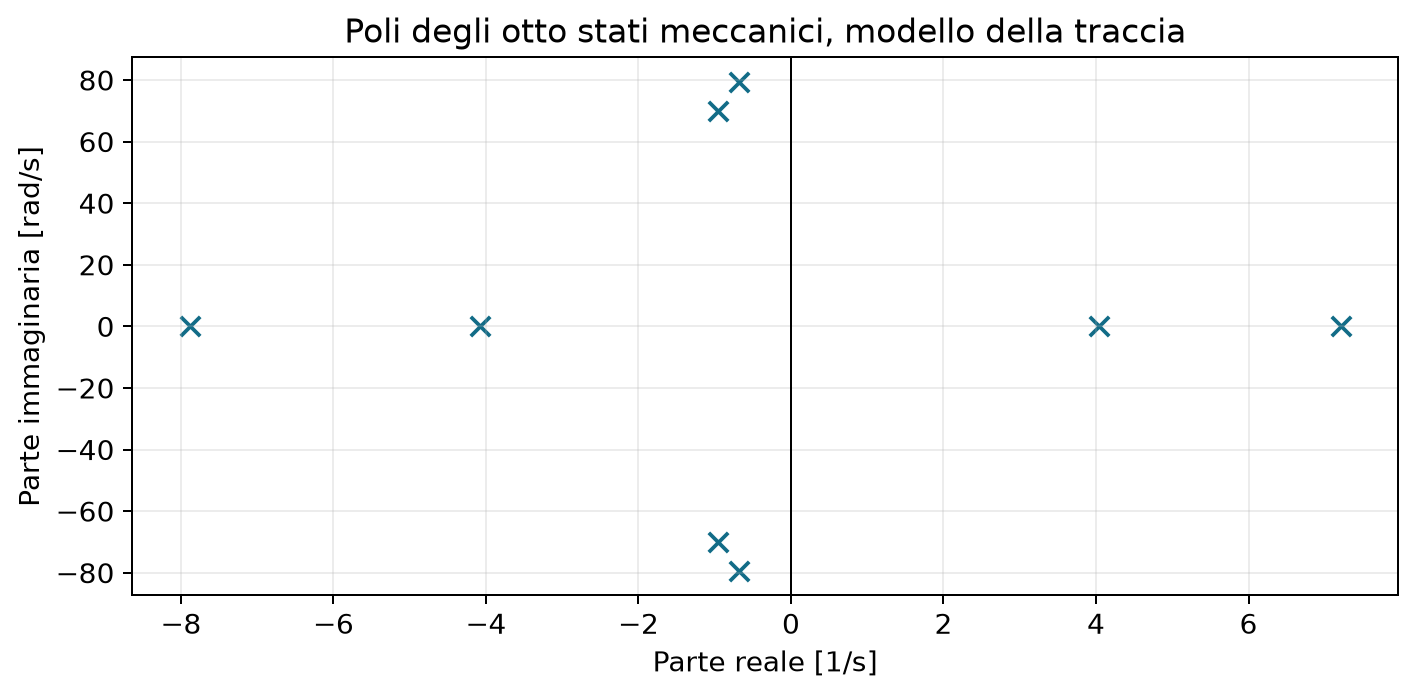
\includegraphics[width=.85\linewidth]{figures/editoriale/poli_meccanici.png}
\caption{Spettro della matrice meccanica salvata con massa nominale.
I poli reali positivi indicano l'instabilità della postura; le coppie
complesse distinguono i modi elastici più rapidi. È una visualizzazione
della linearizzazione disponibile, ricalcolata sul modello corrente.}
\end{figure}

Usiamo il criterio PBH su tutti i modi per verificare che le coppie possano controllarli e che gli encoder possano osservarli. Il modello completo è controllabile e osservabile: i ranghi PBH sono entrambi 14. In particolare è stabilizzabile e rilevabile. Questo è il controllo strutturale necessario alle sintesi; non ricaviamo conclusioni dal solo rango di matrici contenenti alte potenze di $A_m$.

La linearizzazione descrive piccole variazioni attorno all'equilibrio. Per spostamenti maggiori valutiamo direttamente le equazioni non lineari. La stabilità del modello lineare non viene presentata come una garanzia globale sul braccio.

Il criterio PBH controlla se un modo instabile può essere influenzato
dalle coppie e ricostruito dalle misure. Le matrici classiche di
controllabilità e osservabilità contengono alte potenze di $A_m$:
con scale meccaniche e attuative diverse possono essere mal condizionate.
Per le sintesi servono stabilizzabilità e rilevabilità dei modi critici,
non un rango dichiarato senza tolleranza numerica.
Le frequenze elastiche più elevate spiegano inoltre perché aumentare
molto la rapidità del feedback possa richiedere più coppia e rendere
più rilevante l'incertezza dei drive.

